\textbf{Introduction}\\
Au niveau de ce chapitre nous allons développer le deuxième sprint qui va suivre la même démarche que le premier.
\section{Sprint Planning Meeting}
\subsection{Objectif de sprint}
Au cours de ce deuxième sprint, nous allons développer la fonctionnalité suivante: Gestion de formation.\\
Le développement du sprint passe par les étapes suivantes: Analyse, conception et réalisation.
\subsection{Backlog du deuxième sprint}
L'élaboration du deuxième sprint backlog à partir du Backlog product est présentée dans le tableau suivant:
\begin{table}[!h]
	\centering % used for centering table
	\begin{tabular}{|c|p{6cm}|p{6cm}|c|}
		\hline
		\textbf{Id}&\textbf{User Story} & \centering{\textbf{Sprint Backlog Item}} & \textbf{Effort}\tabularnewline
		\hline
		\multirow{3}{*}{US3}&\multirow{3}{6cm}{En tant qu'administrateur, je peux intégrer des formations dans le thème }&Développer un plugin pour créer un nouveau type de contenu&5\\
		\cline{3-4}
		&&Ajouter des formations &2\\
		\cline{3-4}
		&& Réaliser l'interface &3\\
		\hline
		\multirow{3}{*}{US4}&\multirow{3}{6cm}{En tant qu'administrateur, je peux mettre à jour une formation }&Créer un nouveau type de contenu "Programs"&3\\
		\cline{3-4}
		&&Développer le code au niveau du plugin &3\\
		\cline{3-4}
		&&Réaliser l'interface &3\\
		\hline
		\multirow{3}{*}{US5}&\multirow{3}{6cm}{En tant qu'administrateur, je peux consulter la liste des formations}&Créer la fiche d'archive&2\\
		\cline{3-4}
		&&Développer la fonction permettant de manipuler la requête &5\\
		\hline
		\multirow{3}{*}{US6}&\multirow{3}{6cm}{En tant qu'utilisateur, je peux consulter les détails  des formations}&Créer  la relation entre la formation et le thème(custom Fields)&3\\
		\cline{3-4}
		&&Afficher la relation au niveau de l'interface &3\\
			\hline
		
		
		
	\end{tabular}
	\caption{Tableau : Backlog Sprint 2}
\end{table} 
\newpage
\section{Analyse}
\subsection{Diagramme des cas d'utilisation}
\begin{itemize}
	\item Diagramme de cas d'utilisation global du sprint 2
	
	\begin{figure}[!h]
		\centering
		{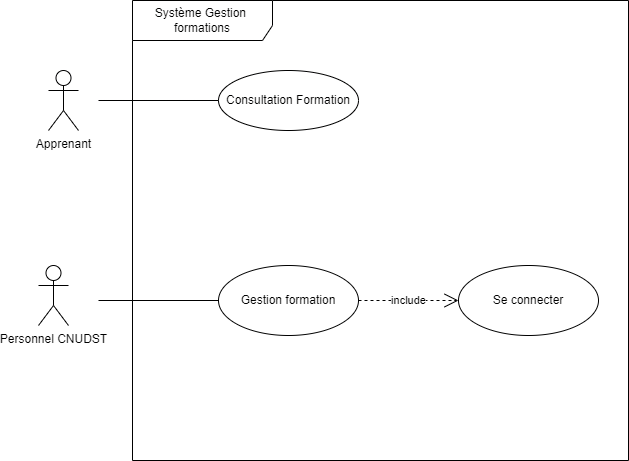
\includegraphics[width=0.75\textwidth]{D) IMAGES/globalformation.png}}
		\caption{Interface :Diagramme du cas d'utilisation global-sprint 2 }
		\label{Org}
	\end{figure}
\newpage
	\item Détails du cas d'utilisation globale<<Gestion formation>>
	
	\begin{figure}[!h]
		\centering
		{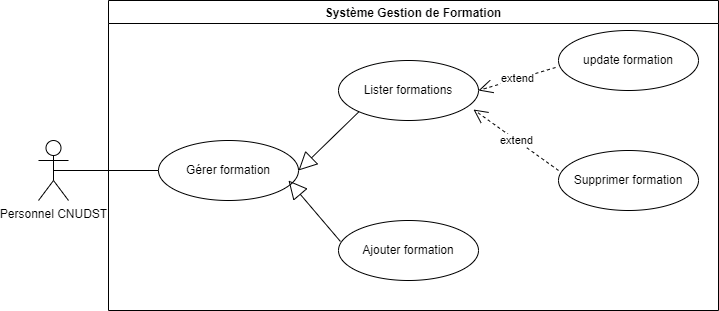
\includegraphics[width=0.95\textwidth]{D) IMAGES/Gestform.png}}
		\caption{Interface :Détails du cas d'utilisation "Gestion formation" }
		\label{Org}
	\end{figure}
\item Détails du cas d'utilisation globale "Consultation formation"

\begin{figure}[!h]
	\centering
	{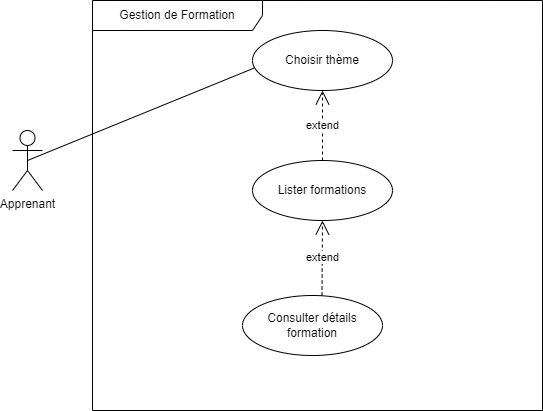
\includegraphics[width=0.75\textwidth]{D) IMAGES/detail2.png}}
	\caption{Interface :Détails du cas d'utilisation "Consultation formation" }
	\label{Org}
\end{figure}
\end{itemize}
\section{Description textuelle des cas d'utilisation}
\subsection{Cas d'utilisation "Consulter formation"}
\textbf{Description textuelle du cas d'utilisation : Consulter formation}\\
\textbf{Titre :} Cas d'utilisation: consulter formation\\
\textbf{But:} Citer les étapes permettant à un visiteur de consulter la liste et les détails des formations fournies par le CNUDST.\\
\textbf{Acteur Principal:} visiteur\\
\textbf{Date de création:} 19/07/2022\\
\textbf{Date de mise à jour:} 21/07/2022\\
\textbf{Responsable:} Olfa CHAOUECH\\
\textbf{Version:} 1.0\\
\textbf{Description des scénarii:}\\
Le cas d'utilisation commence quand un visiteur est connecté au site web et il est sur la page d'accueil.

	 \textbf{Pré condition:}\\
	Le visiteur est sur notre page d'accueil.\\
	\textbf{Scénario nominal:}
	\begin{enumerate}
		\item Le visiteur choisit un thème et clique dessus.
		\item le système affiche la liste de toutes les formations liées au thème choisi.
		\item le visiteur choisit une formation et clique dessus.
		\item le système affiche les détails de cette formation.

    \textbf{Scénario Alternatif A:}\\
    A1 : Le visiteur est sur la page de formations(Programs) et veut consulter les autres formations disponibles.
    $\rightarrow$ L'enchaînement A1 démarre au point 4 du scénario nominal.
    \item Le visiteur clique sur le thème et revient à la liste des formations.
    $\rightarrow$ Le scénario reprend au point 2.
    
\textbf{Scénario d'exception E:}\\
E1 : Le visiteur ne trouve pas la formation souhaitée.
$\rightarrow$ L'enchaînement E1 démarre au point 2 du scénario nominal.

\item Le visiteur termine sa visite en quittant la page.
\end{enumerate}
\textbf{Post-condition:}
Le visiteur a consulté les détails des formations.
\subsection{Cas d'utilisation "Ajouter formation"}
\textbf{Description textuelle du cas d'utilisation : Ajouter formation}\\
\textbf{Titre :} Cas d'utilisation: ajouter formation\\
\textbf{But:} Détailler les étapes permmettant à un administrateur d'ajouter une ou plusieurs formations.\\
\textbf{Acteur Principal:} administrateur\\
\textbf{Date de création:} 15/06/2022\\
\textbf{Date de mise à jour:} 24/06/2022\\
\textbf{Responsable:} Olfa CHAOUECH\\
\textbf{Version:} 1.0\\
\textbf{Description des scénarii:}\\
Le cas d'utilisation commence quand l'administrateur est connecté et il est sur la page de menu de Wordpress.

\textbf{Pré condition:}\\
L'administrateur est sur la page de menu de wordpress.\\
\textbf{Scénario nominal:}
\begin{enumerate}
	\item L'administrateur clique sur le type de contenu Programs.
	\item Le système affiche un menu pour ajouter une formation. 
	\item L'administrateur remplit les champs.
	\item L'administrateur clique sur le bouton ajouter.
	
	\textbf{Scénario Alternatif A:}\\
	A1 : L'administrateur est sur la page de menu et veut ajouter une autre formation.
	$\rightarrow$ L'enchaînement A1 démarre au point 3 du scénario nominal.
	
	
	\textbf{Scénarion d'exception E:}\\
	E1 : L'administrateur ne remplit pas les champs.
	$\rightarrow$ L'enchaînement E1 démarre au point 3 du scénario nominal.
	
	\item L'administrateur ajoute l'ensemble des formations et quitte la page.
\end{enumerate}
\textbf{Post-condition:}
Toutes les formations ont été ajoutées par l'administrateur.
\subsection{Cas d'utilisation "Lister formation"}
\textbf{Description textuelle du cas d'utilisation : Lister formation}\\
\textbf{Titre :} Cas d'utilisation: lister formation\\
\textbf{But:} Détailler les étapes permettant à un administrateur d'afficher la liste des formations.\\
\textbf{Acteur Principal:} administrateur\\
\textbf{Date de création:} 28/06/2022\\
\textbf{Date de mise à jour:} 01/07/2022\\
\textbf{Responsable:} Olfa CHAOUECH\\
\textbf{Version:} 1.0\\
\textbf{Description des scénarii:}\\
Le cas d'utilisation commence quand l'administrateur est connecté et il est sur la page de menu de Wordpress.

\textbf{Pré condition:}\\
L'administrateur est sur la page de menu de wordpress.\\
\textbf{Scénario nominal:}
\begin{enumerate}
	\item L'administrateur clique sur le type de contenu Programs puis sur ALL Programs .
	\item Le système récupère les données des formations de la base. 
	\item Le système affiche la liste de toutes les formations disponibles et en face de chacune il existe deux options: un choix pour "Edit" et un choix pour "Delete" une formation.
	\item L'administrateur consulte la liste des formations.
	\item L'administrateur choisit une formation et choisit une option.
	\item Modification
	\begin{itemize}
		\item L'administrateur clique sur "edit";
		\item Le système affiche une interface de mise à jour d'une formation;
		\item L'administrateur modifie les champs désirés;
		\item L'administrateur clique sur update;
		\item Le système met à jour les données de la formation dans la base;
	\end{itemize}
	
	\item Suppression
	\begin{itemize}
		\item L'administrateur clique sur "delete";
		\item Le système affiche un message de confirmation;
		\item L'administrateur confirme la suppression;
	\end{itemize}
	
	\textbf{Scénario Alternatif A:}\\
	A1 : L'administrateur est sur la page de mise à jour d'une formation et veut modifier une autre.
	$\rightarrow$ L'enchaînement A1 démarre au point 3 du scénario nominal
	.
	
	
	\textbf{Scénario d'exception E:}\\
	E1 : L'administrateur change d'avis et veut abandonner la consultation des formations et les opérations de modification et de suppression.
	$\rightarrow$ L'enchaînement E2 démarre au point 3 du scénario nominal.
	
	\item L'administrateur quitte la page.
\end{enumerate}
\textbf{Post-condition:}
L'administrateur effectue les modifications désirées.
\section{Conception}
\subsection{Diagramme des séquences}
\newpage
\begin{itemize}
	
	\item Diagramme de séquence "Consulter formations"
	\begin{figure}[!h]
		\centering
		{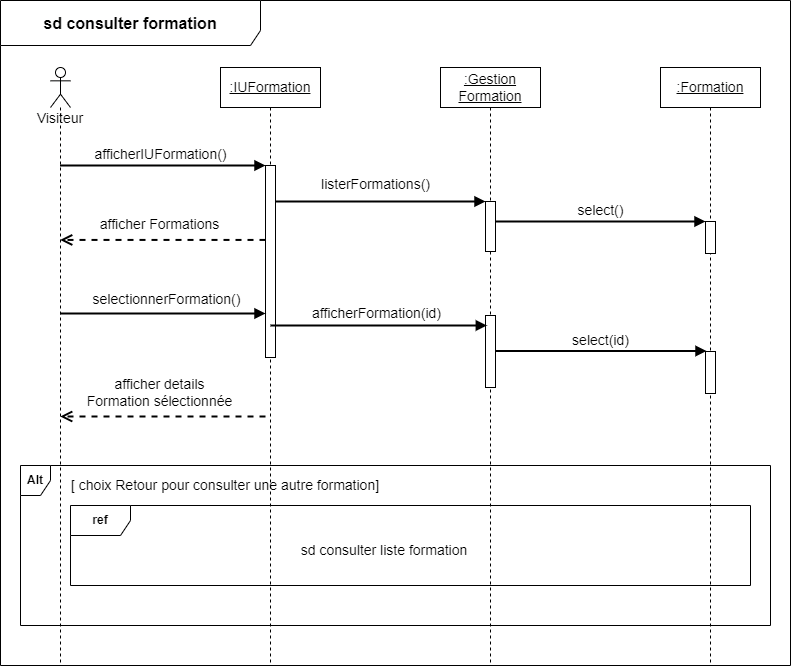
\includegraphics[width=1\textwidth]{D) IMAGES/seqconfor.png}}
		\caption{diagramme de séquence: consulter formation}
		\label{Diagramme3}
	\end{figure}

\newpage




\item Diagramme de séquence "ajouter formation"

\begin{figure}[!h]
	\centering
	{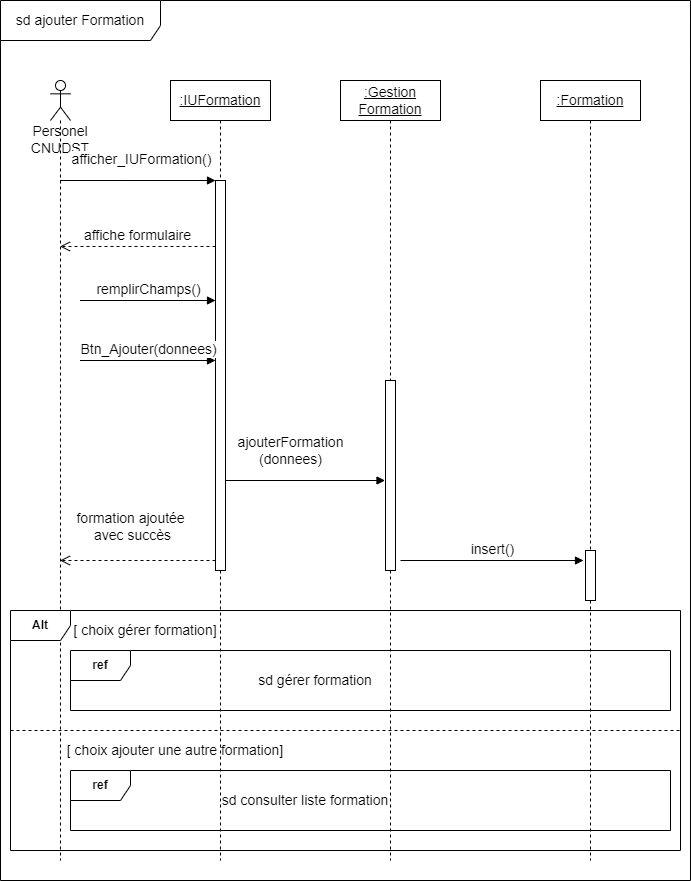
\includegraphics[width=0.95\textwidth]{D) IMAGES/seqform2.png}}
	\caption{diagramme de séquence: ajouter formation}
	\label{Diagramme3}
\end{figure}
\newpage
\item Diagramme de séquence "lister formations"
\begin{figure}[!h]
	\centering
	{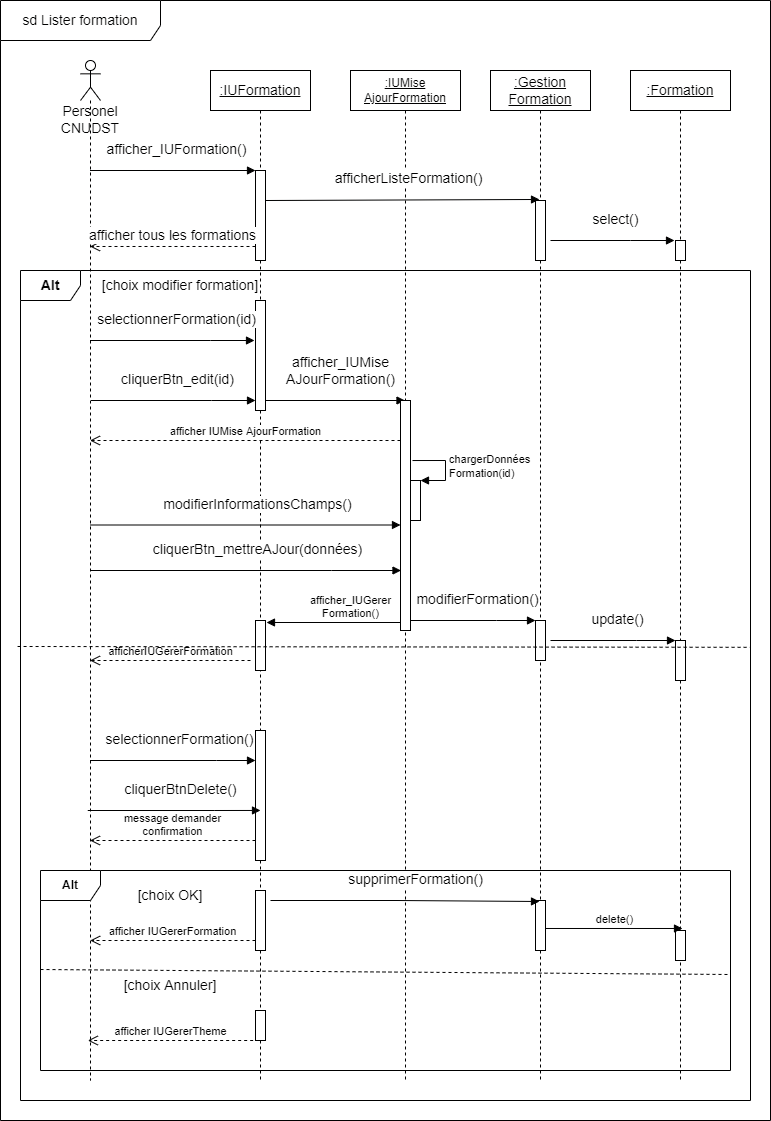
\includegraphics[width=0.75\textwidth]{D) IMAGES/seqforlist.png}}
	\caption{diagramme de séquence: lister formations}
	\label{Diagramme3}
\end{figure}
\newpage
\end{itemize}
\subsection{Diagramme de classes}
La figure ci-dessous correspond au diagramme de classes de notre site, elle représente ses classes, ses méthodes, ses associations et ses propriétés.
\begin{figure}[!h]
	\centering
	{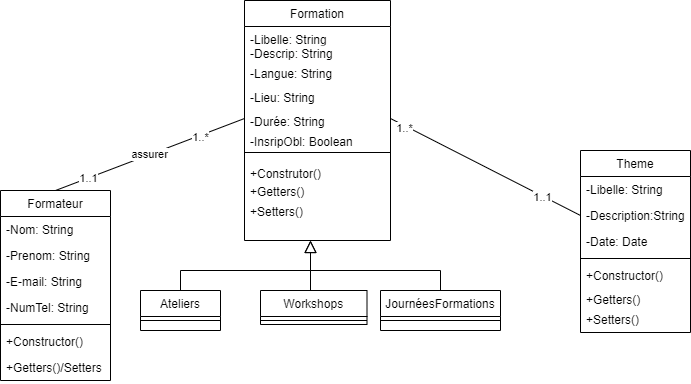
\includegraphics[width=0.75\textwidth]{D) IMAGES/diagClassFor.png}}
	\caption{diagramme de classes sprint 2}
	\label{Diagramme3}
\end{figure}
\section{Réalisation}
\subsection{Description des interfaces}
\begin{itemize}
	\item \textbf{Interface : Interface de la page d'accueil}
	\newpage
	\begin{figure}[!h]
		\centering
		{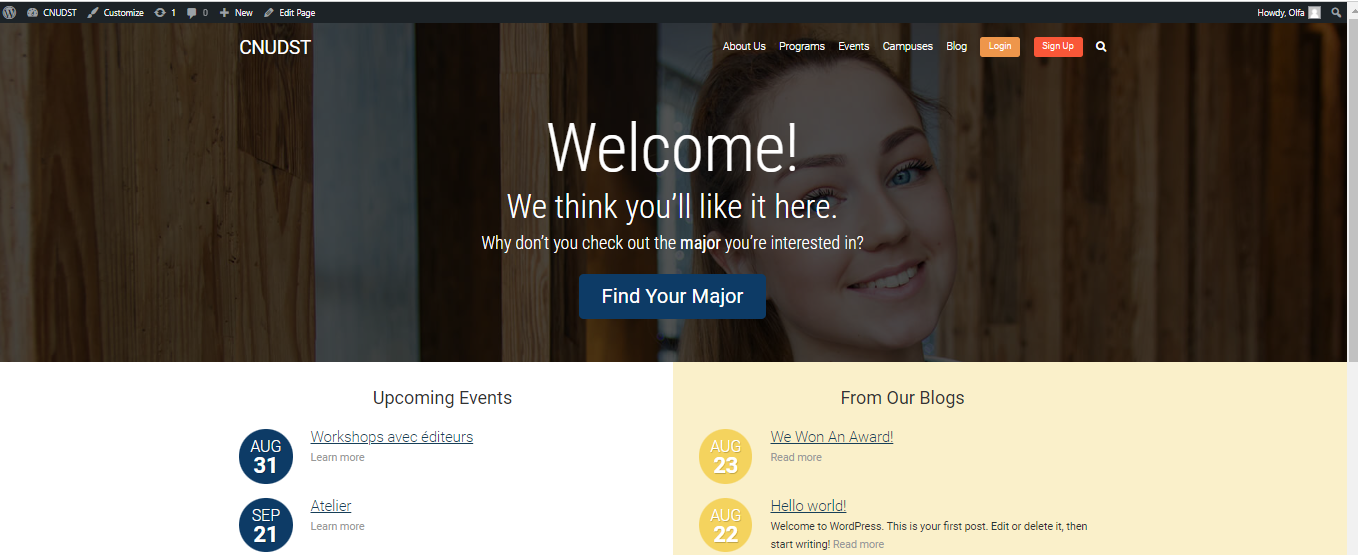
\includegraphics[width=1.05\textwidth]{D) IMAGES/them.png}}
		{
\includegraphics[width=1.05\textwidth]{D) IMAGES/them2.png}}
		\caption{Interface de la page d'accueil}
		\label{Org}
	\end{figure}
	Cette page est la première qui s'affiche quand l'utilisateur visite notre site. Elle lui permet d'avoir une idée sur les thèmes de formations futures (Upcoming Events).
	En cliquant sur le bouton "Find your Major", le visiteur peut lister les formations organisées par le CNUDST.\\
	Sur cette page le visiteur trouve une barre de menu qui lui permettra de naviguer vers les différentes pages du site.\\
	\newpage
	\textbf{Interface: Consultation de la liste des thèmes}\\
	Cette page permet au visiteur d'afficher la liste des thèmes (All Events), aussi elle contient un lien qui permet d'afficher l'ensemble des évènements passés.\\
	\begin{figure}[!h]
		\centering
		{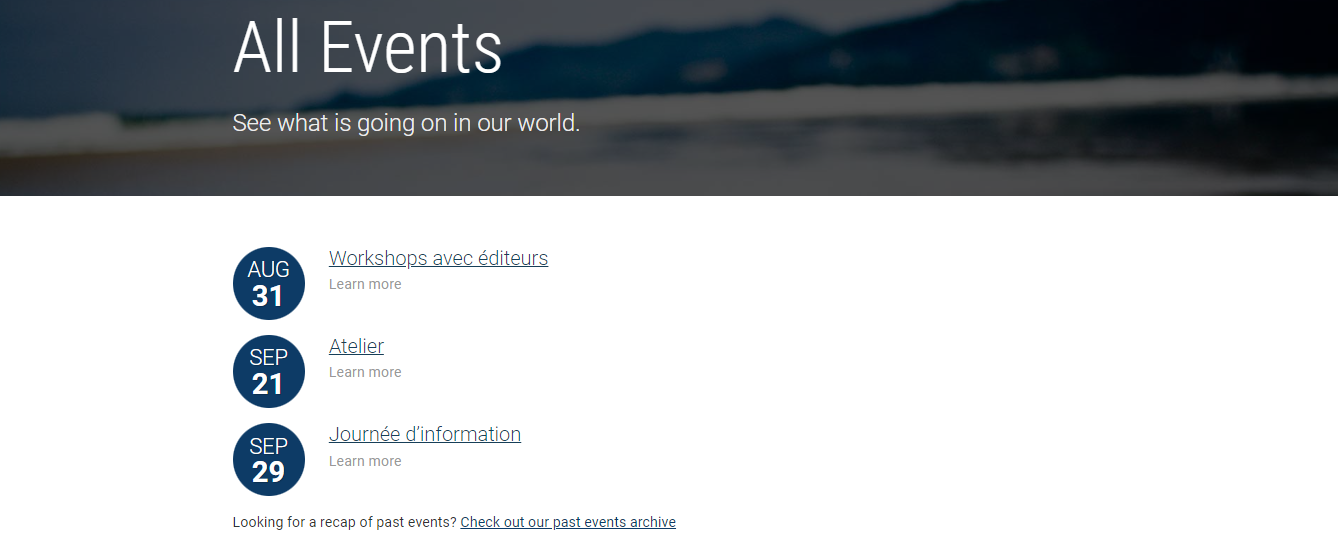
\includegraphics[width=1.05\textwidth]{D) IMAGES/listevent.png}}
		\caption{Interface : Consultation de la liste des thèmes }
		\label{Org}
	\end{figure}\\
	\textbf{Interface: Consultation de la liste des formations}\\
	Cette page permet d'afficher la liste des formations qui vont être organisées par le CNUDST.
	\begin{figure}[!h]
		\centering
		{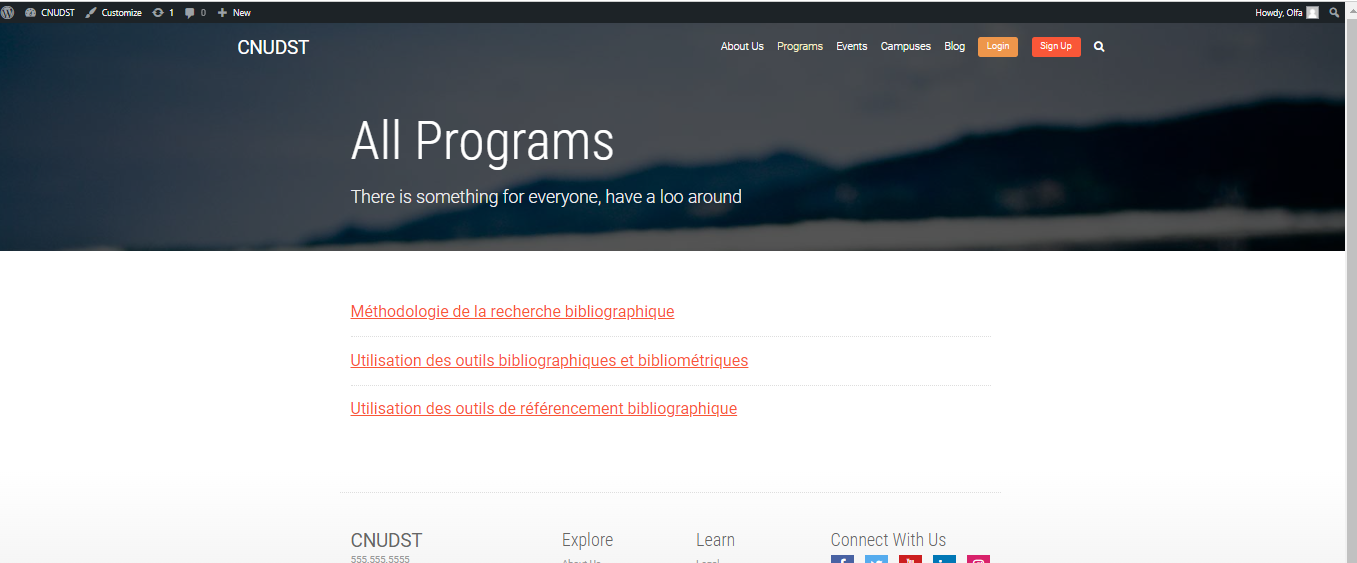
\includegraphics[width=1.05\textwidth]{D) IMAGES/allprog.png}}
		\caption{Interface : Consultation de la liste des formations }
		\label{Org}
	\end{figure}\\
\newpage
	\textbf{Interface : Détails formations}\\
	\begin{figure}[!h]
		\centering
		{
\includegraphics[width=1.05\textwidth]{D) IMAGES/detfor.png}}
		{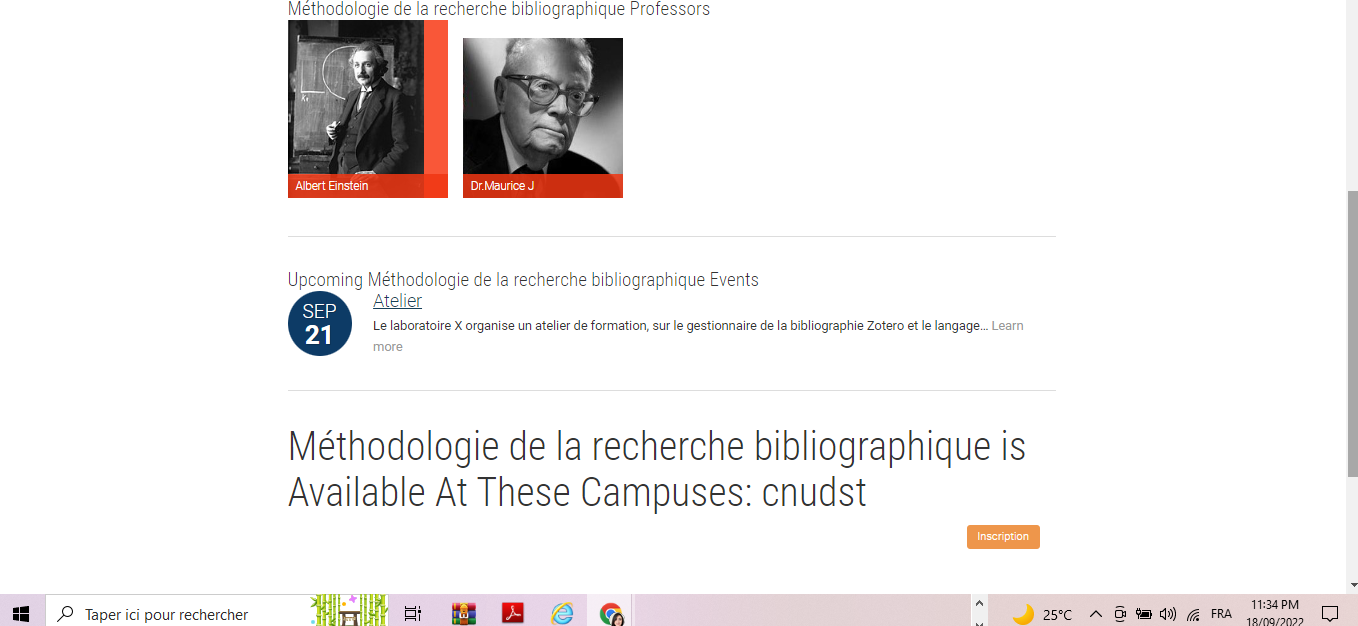
\includegraphics[width=1.05\textwidth]{D) IMAGES/detfor2.png}}
		{
\includegraphics[width=1.05\textwidth]{D) IMAGES/detfor3.png}}
		\caption{Interface : détails formations}
		\label{Org}
	\end{figure}
	Cette page permet au visiteur de consulter les détails d'une formation. \\
	\textbf{Interface : Gérer les formations par l'administrateur (lister, ajouter, modifier et supprimer)}\\
	C'est une interface qui permet à l'administrateur d'ajouter, lister, modifier et supprimer une formation.
	\newpage 
	\begin{figure}[!h]
		\centering
		{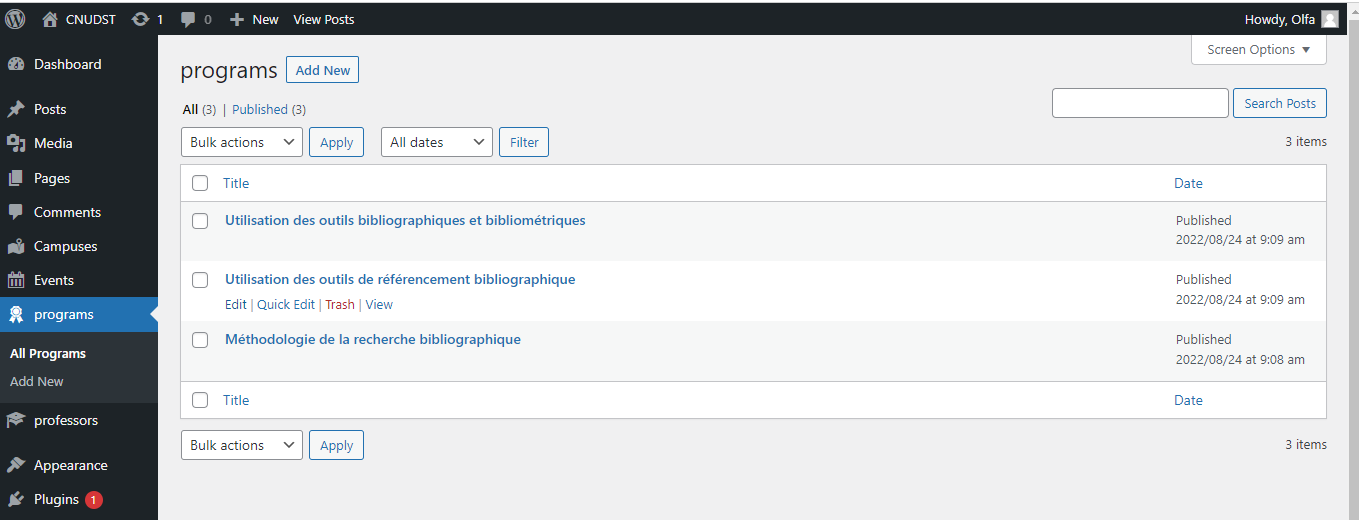
\includegraphics[width=1.05\textwidth]{D) IMAGES/Gerer.png}}
		\caption{Interface : Gérer les formations par l'administrateur }
		\label{Org}
	\end{figure}
\end{itemize}
\textbf{Conclusion}\\
Dans ce chapitre, nous avons essayé de mettre le focus sur le développement du deuxième sprint qui a duré quatre semaines.\\
Dans ce qui suit, nous allons entamer le dernier sprint de notre processus de développement des EPIC: \begin{itemize}
	\item Inscription à une formation en lige
	\item Interaction sur le site
\end{itemize}.





